
\usetikzlibrary{positioning, arrows.meta}


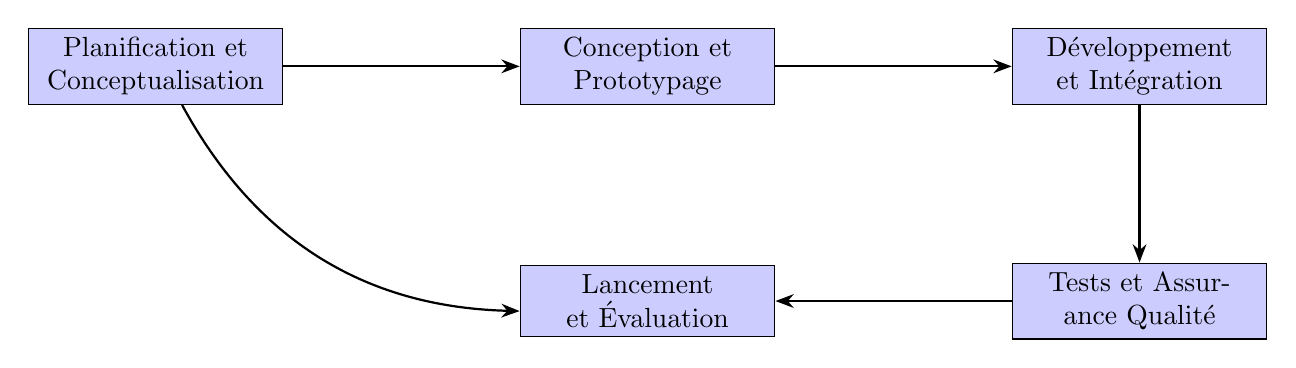
\begin{tikzpicture}[
	node distance=2cm and 3cm,
	milestone/.style={rectangle, draw, fill=blue!20, text width=3cm, align=center},
	arrow/.style={-Stealth, thick}
	]
	
	% Milestones
	\node[milestone] (planning) {Planification et Conceptualisation};
	\node[milestone, right=of planning] (design) {Conception et Prototypage};
	\node[milestone, right=of design] (development) {Développement et Intégration};
	\node[milestone, below=of development] (testing) {Tests et Assurance Qualité};
	\node[milestone, left=of testing] (launch) {Lancement et Évaluation};
	
	% Arrows
	\draw[arrow] (planning) -- (design);
	\draw[arrow] (design) -- (development);
	\draw[arrow] (development) -- (testing);
	\draw[arrow] (testing) -- (launch);
	\draw[arrow] (planning) edge[bend right] (launch);
	
\end{tikzpicture}
